\begin{figure}[htb]\centering
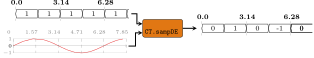
\includegraphics[width=\textwidth]{figs/example-forsyde-plot}
\end{figure}
\lstinputlisting[firstline=4]{figs_src/example-forsyde-plot.tex}
\newpage

\section{The \texttt{forsyde-plot} package}
\label{sec:forsyde-plot-package}


This package provides environments and plot commands for visualizing the contents of \ForSyDe\ signals. It is meant to be an alternative to GNUplot or other plotting tools, but not necessarily a replacement for these. The package is imported using the command \texttt{\char`\\usepackage[plot]\{forsyde\}} in the document preamble.

\subsection{The \texttt{signalsSY} environment}
\label{sec:plot-signalsSY}


This environment creates a \textsc{TikZ} matrix of events, where each row is the content of a signal, and ``synchronous'' events are aligned on columns. This environment is suitable for depicting signals where the time/causality between events is implicit from their position in the signal. This includes synchronous signals, but also any dataflow signals.

\bookmark{environment}
\begin{verbatim}
\begin{signalsSY}[options]

  body...
\end{signalsSY}
\end{verbatim}

The \texttt{body} of the environment usually consists of a series of \texttt{\char`\\signalSY} commands, but it may also contain any command acceptable within a \textsc{TikZ} \texttt{matrix} environment. Notice that it needs an initial line break. The \texttt{options} are:

\bookmark{options}
\begin{optionslist}
\item \texttt{name=} the name of the \textsc{TikZ} element. Default is \texttt{sigplot}.
\item \texttt{at=} the position of the plot within the \texttt{tikzpicture}. Default is \texttt{(0,0)}.
\item \texttt{xshift=\it dist}, \texttt{yshift=\it dist}, \texttt{shift=\it coord} a displacement in the respective direction.
\item \texttt{anchor=\it anchor} where this element should be anchored.
\item \texttt{left of=\it coord}, \texttt{right of=\it coord}, \texttt{above of=\it coord}, \texttt{below of=\it coord} positions the element accordingly.
\item \texttt{inputs=\it coord}, \texttt{outputs=\it coord} positions the element left of/right of the given coordinate.
\end{optionslist}

\begin{figure}[htb]\centering
\includegraphics{figs/example-signal-sy}
\lstinputlisting[linerange={9-14}]{figs_src/example-signal-sy.tex}
\caption{The \texttt{\char`\\signalSY} draw command. The red boxes are nodes accessed with \texttt{[name]-[row]-[column]}.}
\end{figure}
\hspace{1pt}\bookmark{\char`\\signalSY\man{\{events\}}}

\noindent The SY signal is simply a row in a matrix, and the elements can be accessed according to the \textsc{TikZ} matrix of nodes.

\subsection{The \texttt{signalsDE} environment}
\label{sec:plot-signalsDE}

This environment creates a (simple) plot of DE signals similar to Modelsim or GTKwave, within a \texttt{tikzpicture}.

\bookmark{environment}
\begin{verbatim}
\begin{signalsDE}[options]{xmax}
  body...
\end{signalsDE}
\end{verbatim}

The body within the environment consists of a series of \texttt{\char`\\signalDE} commands. It \emph{requires} an \texttt{xmax} number which stands for the last timestamp plotted. The \texttt{options} are:

\bookmark{options}
\begin{optionslist}
\item \texttt{name=} the name of the \textsc{TikZ} element. Default is \texttt{sigplot}.
\item \texttt{grid=\it step} draws a dashed line every \texttt{step} time(stamps).
\item \texttt{timestamp=\it step} shows the time(stamp) above the plot at every \texttt{step}.
\item \texttt{grid and time=\it step} is equivalent to \texttt{grid=\it step} and \texttt{timestamp=\it step}.
\item \texttt{label pos=} position of the label within the plotted bar. Default is \texttt{center}.
\item \texttt{signal sep=\it dist} the vertical distance between two consecutive signals.
\item \texttt{xscale=\it ratio} and \texttt{yscale=\it ratio} scales the plot.
\item \texttt{at=} the position of the plot within the \texttt{tikzpicture}. Default is \texttt{(0,0)}.
\item \texttt{xshift=\it dist}, \texttt{yshift=\it dist}, \texttt{shift=\it coord} a displacement in the respective direction.
\item \texttt{anchor=\it anchor} where this element should be anchored.
\item \texttt{left of=\it coord}, \texttt{right of=\it coord}, \texttt{above of=\it coord}, \texttt{below of=\it coord} positions the element accordingly.
\item \texttt{inputs=\it coord}, \texttt{outputs=\it coord} positions the element left of/right of the given coordinate.
\end{optionslist}

\begin{figure}[htb]\centering
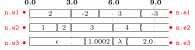
\includegraphics{figs/example-signal-de}
\lstinputlisting[linerange={7-10,13-17}]{figs_src/example-signal-de.tex}
\caption{The \texttt{\char`\\signalDE} draw command. The red dots are custom anchors accessed with \texttt{[name]-[anchor]}.}
\end{figure}
\hspace{1pt}\bookmark{\char`\\signalDE\opt{*}\opt{[options]}\man{\{events\_or\_datafile\}}}

\noindent The DE signal command has two versions: a starred (\texttt{*}) version taking as argument the path to a file containing the input data, or the non-starred version which takes as argument the actual data (events). In both cases the data needs to be formatted as

\begin{verbatim}
value1 : timestamp1, value2 : timestamp2, ... , valueN : timestampN
\end{verbatim}

\noindent where \texttt{timestampN} $>$ \texttt{xmax}. The \texttt{options} are:

\begin{optionslist}
\item \texttt{name=} the name of the signal.
\item \texttt{trunc} a flag activating value truncation to integers. Works only of all values of a signal are numbers. Default is \texttt{false}.
\item \texttt{last label} a flag enabling the last value in a signal to be printed or not. Default is \texttt{true}.
\end{optionslist}


\subsection{The \texttt{signalsCT} environment}
\label{sec:plot-signalsDE}

This environment creates a (simple) stacked plot of CT signals within a \texttt{tikzpicture}.

\bookmark{environment}
\begin{verbatim}
\begin{signalsCT}[options]{xmax}
  body...
\end{signalsCT}
\end{verbatim}

The body within the environment consists of a series of \texttt{\char`\\signalCT } commands. It \emph{requires} an \texttt{xmax} number which stands for the last timestamp plotted. The \texttt{options} are:

\bookmark{options}
\begin{optionslist}
\item \texttt{name=} the name of the \textsc{TikZ} element. Default is \texttt{sigplot}.
\item \texttt{grid=\it step} draws a dashed line every \texttt{step} time(stamps).
\item \texttt{timestamp=\it step} shows the time(stamp) above the plot at every \texttt{step}.
\item \texttt{grid and time=\it step} is equivalent to \texttt{grid=\it step} and \texttt{timestamp=\it step}.
\item \texttt{label pos=} position of the label within the plotted bar. Default is \texttt{center}.
\item \texttt{signal sep=\it dist} the vertical distance between two consecutive signals.
\item \texttt{xscale=\it ratio}, \texttt{yscale=\it ratio} scales the plot.
\item \texttt{at=} the position of the plot within the \texttt{tikzpicture}. Default is \texttt{(0,0)}.
\item \texttt{xshift=\it dist}, \texttt{yshift=\it dist}, \texttt{shift=\it coord} a displacement in the respective direction.
\item \texttt{anchor=\it anchor} where this element should be anchored.
\item \texttt{left of=\it coord}, \texttt{right of=\it coord}, \texttt{above of=\it coord}, \texttt{below of=\it coord} positions the element accordingly.
\item \texttt{inputs=\it coord}, \texttt{outputs=\it coord} positions the element left of/right of the given coordinate.
\end{optionslist}

\begin{figure}[htb]\centering
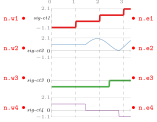
\includegraphics{figs/example-signal-ct}
\lstinputlisting[linerange={9-22}]{figs_src/example-signal-ct.tex}
\caption{The \texttt{\char`\\signalCT} draw command. The red dots are custom anchors accessed with \texttt{[name]-[anchor]}.}
\end{figure}
\hspace{1pt}\bookmark{\char`\\signalCT\opt{*}\opt{[options]}\man{\{events\_or\_datafile\}}}

\noindent The CT signal command has two versions: a starred (\texttt{*}) version taking as argument the path to a file containing the input data, or the non-starred version which takes as argument the actual data (events). In both cases the data needs to be formatted as

\begin{verbatim}
value1 : timestamp1, value2 : timestamp2, ... , valueN : timestampN
\end{verbatim}

\noindent where \texttt{timestampN} $>$ \texttt{xmax}. The \texttt{options} are:

\begin{optionslist}
\item \texttt{name=} the name of the signal.
\item \texttt{ordinate=} draws the X axis (ordinate) on the value passed as argument.
\item \texttt{outline} a flag for drawing the outline for a signal. Default is \texttt{false}.
\item \texttt{ymax=\it num}, \texttt{ymin=\it num} the maximum and minimum values covered by the plot. Default is \texttt{ymin=0} and \texttt{ymax=1}.
\item \texttt{line style=} a style passed to the drawing tool.
\end{optionslist}

\newpage
\vspace*{\fill}%

%%% Local Variables:
%%% TeX-command-default: "Make"
%%% mode: latex
%%% TeX-master: "../refman"
%%% End:
